
\section{Internet felderítő projektek} \label{internet-measurement}

%(6 oldal): CAIDA, Archipelago és egyéb mérőrendszerek, PlanetLab, útvonal eltérítések esetei


Jelen fejezetben a legfontosabb Internet felderítését célzó szervezeteket és projekteket ismertetem, illetve megemlítem a legfontosabb ezeket felhasználó cikkeket.


\subsection{Internet elemző központ: CAIDA}

%\textbf{2-3 oldal kb}

A CAIDA (Center for Applied Internet Data Analysis)\footnote{\url{http://www.caida.org/home/}} egy kollaborációs együttműködése állami, kutatói és kereskedelmi szervezeteknek aminek célja az Internet üzemeltetésének, felügyeletének és fejlesztésének segítése. Alapvetően az alábbi három fő területre koncentrálódnak a szervezet munkakörei és projektjei:

\begin{itemize}
\item Kutatás és analizálás
%Research and Analysis	Analyze
\item Mérés és infrastruktúra
%Measurements and Infrastructure
\item Adat és eszközök.
%Data and Tools.
\end{itemize}

Munkájuk során az Internet egyes aspektusainak megismeréséhez modelleket készítenek, majd vizsgálják azok érvényességét, végül publikálják a talált összefüggéseket. Céljuk előremozdítani az Internet növekedésének problémamentességét. Ennek érdekében folyamatosan feltérképezik az Internet szerkezetét, amelyet a korábbi fejezetekben is bemutattam. Évente új \mbox{\glqq térképet \grqq} készítenek az Autonóm Rendszerek hálózatáról, mind az IPv4, mind az IPv6-os hálózatrészekről külön-külön. A \ref{fig:caida-poster} ábrán látható gráf pontjainak (AS) elhelyezése a földön is betöltött szélességi foka alapján (irány) és a rajta átmenő linkek száma alapján vannak elhelyezve (sugár, logaritmikusan ábrázolva).

\begin{figure}[!ht]
	\centering
	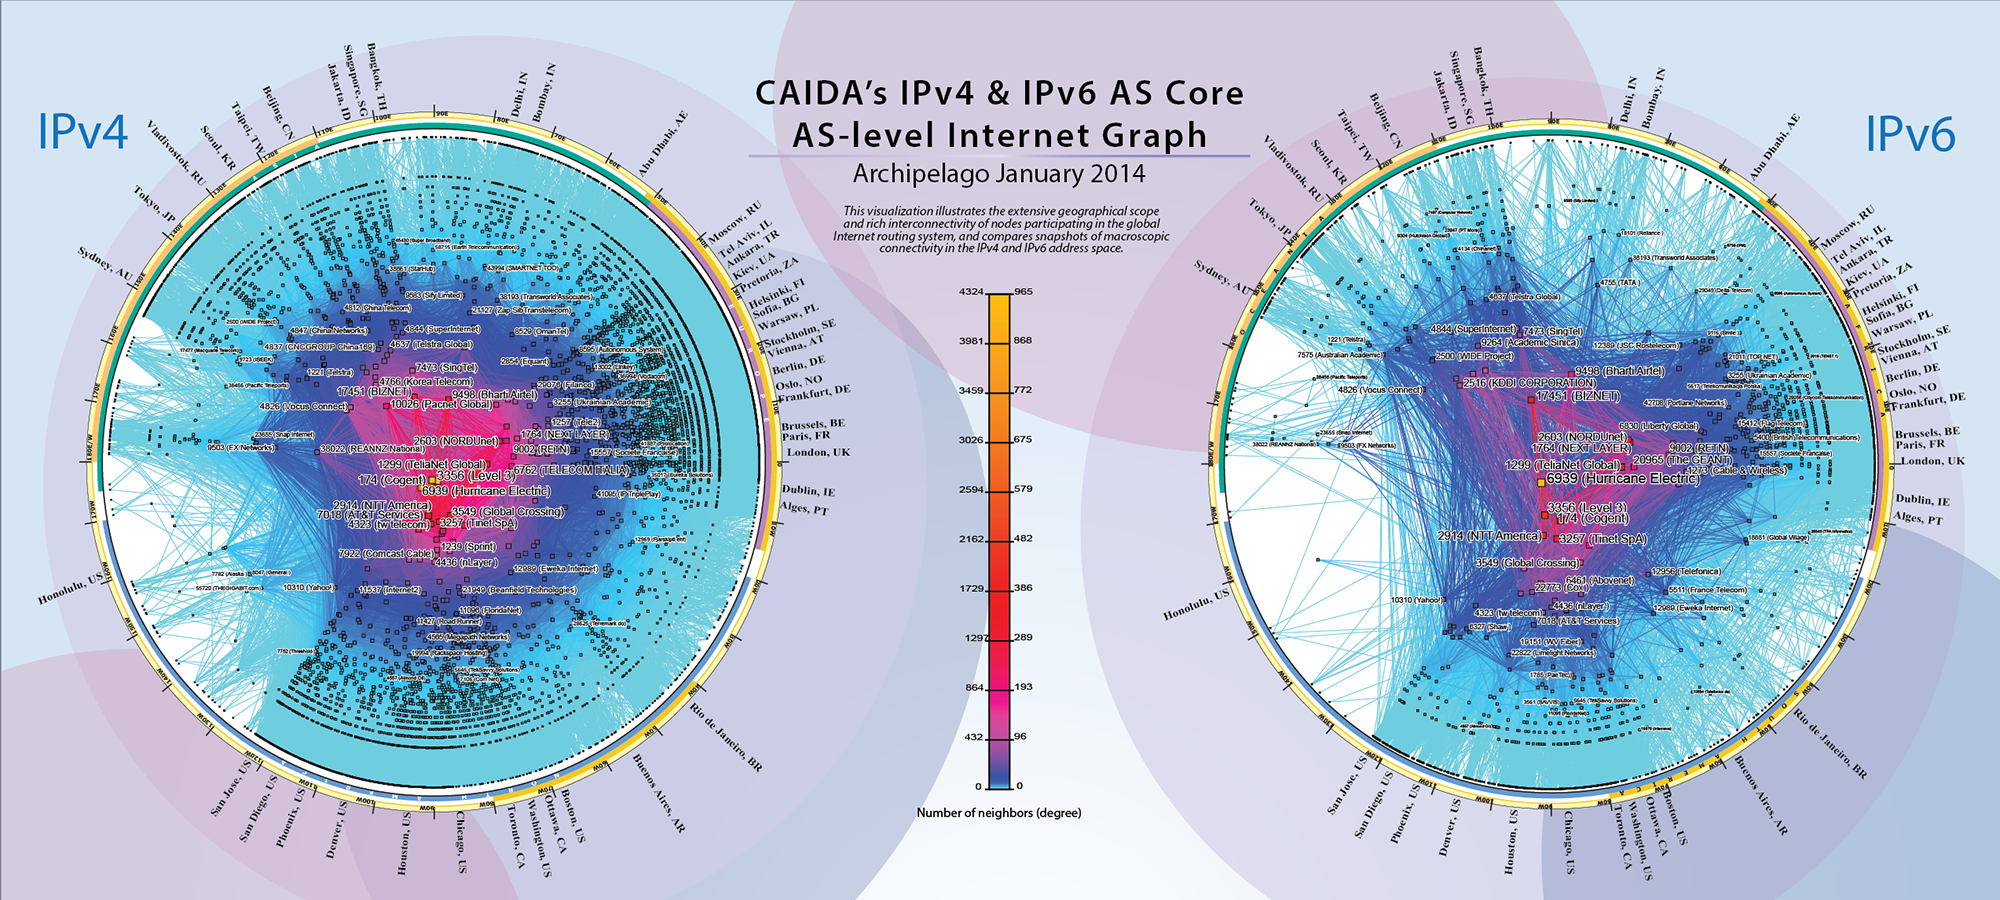
\includegraphics[width=0.9\textwidth, keepaspectratio]{figures/caida-poster.png}
	\caption{Az Internet AS gráfja 2014-ben}
	\label{fig:caida-poster}
\end{figure}

Az általános megfigyeléseken felül kutatásaik a kibervédelemre is kiterjednek. Céljuk az Internet helyes működése elleni tevékenységek felderítése és utólagos megértésük.


Ezen széles skálájú megfigyelésekhez kiterjedt mérési rendszereket üzemeltetnek a világ minden táján. Többek között begyűjtik az összes publikusan elérhető BGP útvonalhirdetéseket és a kooperáló szervezeteknél elhelyezkedő traceroute szerverekkel felméréseket végeznek a csomagtovábbítási viszonyokról az Internet egyes részeiben. Mindezeken felül pedig több Autonóm Rendszer hálózatában passzív méréseket is végeznek. Ennek a felhasználására egy példa az internetes háttérzaj mérése, ami az olyan adatcsomag küldések intenzitását mérik, amelyek olyan cél címekkel rendelkeznek ahol nem létezik fogadó számítógép. Az ilyen csomagok általában botnetek terjedési próbálkozásának a terméke.

Az említett adatforrások egy központi gyűjtő és organizáló rendszerbe, az ARK\footnote{Archipelago}-ba vannak csatornázva. A feldolgozás során rendkívül nagy hangsúly van fektetve a kinyert adatok hivatalosításán. Minden származtatott adatban meg vannak jelölve annak forrásai, valamint a különböző forrásokból származó azonos információk gondosan össze vannak vetve, ellenőrizve megbízhatóságukat.

%további tartalom majd innen: http://www.caida.org/home/about/progplan/progplan2014/
%% fél oldal kb eddig

%második oldal a 3 fő tématerületének a kifejtése, témánként fél oldal.

%Számunkra legfontosabb.. felsorolás a projektjeik közül

%%%%%%%%%%%%%%%%%%%%%%%%%%%%%%%%%%%%%%%%%%%%%%

\subsection{PlanetLab}

A PlanetLab konzorcium egyetemi, ipari és kormányzati intézmények együttműködő csoportja, amelyek erőforrásaikat megosztják kutatási céllal, így építik és fejlesztik a PlanetLab számítógépes hálózatát. A résztvevő szervezetek így hozzáférnek a sajátjuknál nagyobb hálózathoz. Ilyen módon a résztvevők kivételes lehetőséghez jutnak, hogy  nagyméretű hálózatokon és elosztott rendszereken tudjanak vizsgálatokat végezni.

A konzorciumot 2002-ben alapította 10 amerikai egyetem az Intel Research közreműködésével, kezdetben 100 számítógép-csomópont létrehozásával. A közösségi teszthálózat évről évre bővült újabb egyetemek és ipari kapcsolatok csatlakozásával. A PlanetLab 2004-ben több Amerikán kívüli szervezetet is befogadott többek között európából, brazíliából és ázsiából. Ebben az évben így már világméretűvé nőtt és több mint 400 számítógép csomóponttal rendelkezett. Napjainkban ez a szám már túllépte az ezret és az \ref{fig:planetlab} ábrán látható, hogy a föld minden táján megtalálhatóak a hálózatban résztvevő csomópontok.

A fejlesztett mérőrendszer is a PlanetLab hálózatát felhasználva végez méréseket az internet szerkezetére vonatkozóan.

\begin{figure}[!ht]
	\centering
	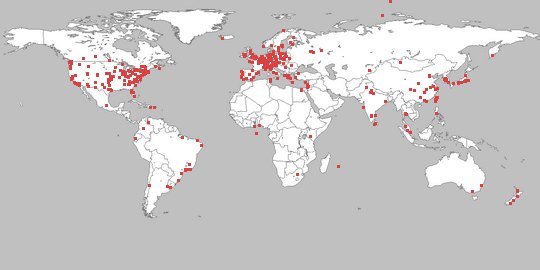
\includegraphics[width=0.65\textwidth, keepaspectratio]{figures/planetlab_worldmap.png}
	\caption{A PlanetLab teszthálózat csomópontjainak elhelyezkedése a világtérképen\label{fig:planetlab}}
\end{figure}

\subsection{M-Lab}
%2 oldal

Az előzőekben bemutatott PlanetLab és további piaci és kutatói szervezetek, többek között a Google, által alakított csoport, melynek célja az Internetes kapcsolatok végfelhasználói szemszögből való elemzése. Egyik legfontosabb célja a felhasználói élmény szűk keresztmetszetének a felderítése.

Begyűjtött adataik fontos része ilyen módon az önkéntes mérésekből származnak. Méréseket a weboldalukról, mobileszközről és telepített szoftverekkel lehet indítani. Minden adatuk nyilvánosan elérhető és letölthető. Több kutatási projektet is támogatnak mérési adataikkal. Naponta több mint 200 ezer tesztet futtatnak, melyek 750 TB adatot gyűjtöttek össze 2015-ig. 


%Elég nagy és működő félig üzleti szervezetnek tűnik. A Google is részese, gondolom ellenőrizni akarják hogy az ISP-k jól működnek-e. Egyik eszközük például külön kutatja, hogy mi a legszűkebb keresztmetszet az ügyfél kapcsolatában.
%Honlapjuk: http://www.measurementlab.net/
%Mobil mérésekkel is foglalkoznak, készítettek egy mobil applikációt ami adatokat gyűjt mérésekről. 2012 és 2013-ban kapott adatok elérhetőek: https://www.measurementlab.net/tools/mobiperf/

\subsection{SamKnows}
%1 oldal

Az Európai Unió és az amerikai FCC is felkarolta az egyetemi projektből kifejlődő SamKnows\footnote{\url{https://www.samknows.com/}} cég működését. Eredetileg a hétköznapi emberek könnyebb és objektív ISP választását segítette a projekt. Kezdetben önkéntesek végeztek méréseket a fejlesztett rendszerükön, hogy megállapítsák a szolgáltatójuk kapcsolatának minőségét. Nem csak sávszélesség mérésre alkalmas, de további hálózati paraméterek mellett a szolgáltatások diszkriminációját is figyeli. Olyan speciális adatcsomagokat használ a mérésekhez, amelyek HTTP, FTP, torrent, youtube, netflix, vagy VOIP\footnote{Voice Over IP - IP alapú hangkapcsolati protokoll} forgalmat szimulálnak. Ezen funkciói miatt rendkívül hasznos ellenőrzési eszköze lett a felügyeleti hatóságoknak. Folyamatosan fejlesztik a rendszerüket és riportokat készítenek a szolgáltatókról és működésükről.
%Az korábbi Internetsemlegességi vitáknál is felhasználták az így gyűjtött adatokat.
Mérési rendszerük támogatja a weboldalon keresztüli méréseket, mobil applikáción keresztüli méréseket és különböző telepíthető hardverelemeket is felhasznál, mint például a SamKnows Whitebox.

\begin{figure}[!ht]
	\centering
	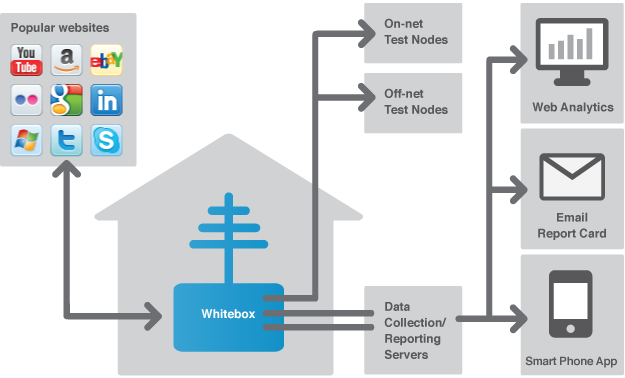
\includegraphics[width=0.45\textwidth, keepaspectratio]{figures/samknows-whitebox.png}
	\hspace{20pt}
	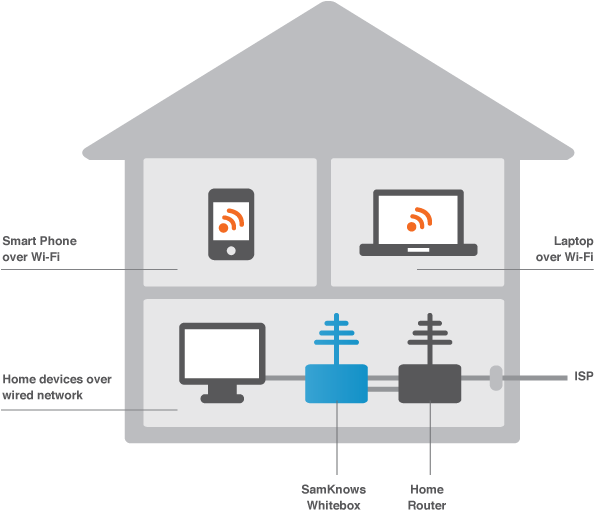
\includegraphics[width=0.45\textwidth, keepaspectratio]{figures/samknows-whitebox2.png}
		
	\caption{A SamKnows Whitebox méréseinek vázlata és elhelyezkedése a háztartásokban}
	\label{fig:samknows}
\end{figure}

A Whitebox készülékek működési elvét a \ref{fig:samknows} ábrák mutatják be, amely a korábban említett méréseket végzi el egy a háztartás hálózatába kötött eszköz segítségével. Az Európia Unió 2012-ben kérte fel a SamKnows céget a tagállamok interneteléréseinek a vizsgálatára. A tanulmány\footnote{\href{https://ec.europa.eu/digital-single-market/news/quality-broadband-services-eu-samknows-study-internet-speeds}{Quality of Broadband Services in the EU}} során 9467 háztartásba helyezték el a Whitebox készülékeket. A mérési adatok publikusan elérhetőek a \url{data.europa.eu} honlapról


\subsection{A DIMES mérési rendszer}
%1.5-2 oldal

2010 és 2013 között több egyetem bevonásával egy Izraeli kutatócsoport indította el a DIMES (Distributed Internet Measurement and Simulation) kutatóprojektet. Céljuk az Internet struktúrájának és topológiájának a megismerése volt, amelyet önkéntes módon segítenek további résztevők.
Az önkéntesek szerepe a geológiai diverzitás volt, amelynek segítségével több megfigyelési pontból lehet megvizsgálni az Internet szerkezetét.
Az elvégzett mérések egyszerű Ping és Traceroute mérésekből álltak, amelyek minimális erőforrásigényt támasztottak az önkéntesek gépein. A résztvevők cserébe személyre szabott jelentéseket kaptak az internetes kapcsolatuk minőségéről.

Kutatási eredményeik felhívták a figyelmet az Autonóm Rendszerek rendkívüli változatosságára és kapcsolataik nehezen felderíthetőségére. Egyik fontos megállapításuk a CAIDA akkori felméréseihez képest, hogy a Looking Glass szervereken keresztül elérhető BGP hirdetésekből hiányoznak az egyes AS-ek peering egyezményeikből fakadó összeköttetések.

A kutatási projekt aktivitása 2013 óta teljesen megszűnt, a hivatalos honlapjuk nincs karbantartva.

%Honlapja: http://www.netdimes.org/new/
%A DIMES honlapja gyakorlatilag nem működik, mindenféle hibákba ütközik (de legalább elérhető). A legutolsó hír rajta vagy bejegyzése 2013-ban íródott. Nem erléhetőek sajnos így az általuk elért adat sem, sem az infók róla :(
%A publikációjukból tudunk legjobban kiindulni: link (2000 és 2013 közöttiek)
%A saját mérési adataik elérhetőek: link
%Lehet érdemes felvenni velük a kontaktot, hogy külsős fél mennyire tudná most futtatni?
%Email: support@netdimes.org
%A projekt résztvevői: link
%A projekt fóruma: link
%A fórumon van egy “friss” szál ahol megbeszélik, hogy ez egy halott projekt (link).
%Ebben a beszélgetésben egy lényegretörő hozzászólás:
%Since I found the project I've now gotten rid of all Windows machines, and the Linux version never worked anyway. I can't run the agent either way.

\subsection{Kisebb Internet mérő projektek}

A fentiekben felsoroltakon kívül még számos kisebb internet mérést célzó projekt létezik még melyek közül a továbbiakban kettőt emelek ki.

\subsubsection*{Az IRL mérési rendszer}
 
 
Egyetemi projektként\footnote{\url{http://irl.cs.tamu.edu/projects/sampling/}} kutatásuk középpontjában a teljes Internetre vonatkozó mérések hatékonyságának a növelése állt. Új eljárásokat fejlesztettek ki, melyekkel nem a bevett elárasztásos módon derítik fel az egyes hálózati tartományokat. Utóbbi publikációjukban\cite{irl-measure} pedig a hálózatban résztvevő eszközök operációs rendszerét állapították meg.
 

%Sampling Internet structure and its service availability have always been important issues in Internet research. This project aims to develop mechanisms for discovering available services in the Internet using scalable end-to-end measurements, facilitate delay sampling between arbitrary hosts using the existing DNS infrastructure, perform more accurate bandwidth estimation, and build router-level maps of the Internet using non-intrusive traceroute to known destinations. We are also working on techniques for fingerprinting OS and server implementations using low-overhead end-to-end methods.


\subsubsection*{Az iPlane mérési rendszer}
 


Diploma munkaként született, majd kutatási projektté fejlődött az iPlane\footnote{\url{http://iplane.cs.washington.edu/}}, melynek fő célja az internetes útvonalak QoS becslése és akár predikciója. Kimutatásaikat a PlanetLab gépeken és további publikus Traceroute szervereken futtatott útvonal felderítő mérések alapján végezték. Céljuk a felhalmozott adatok felhasználása későbbi szolgáltatások minőségének javítására.Elemzéseik fontos része, hogy a felderített útvonalaknak a rész szakaszaira becsülnek paramétereket, így még nem mért útvonalak viselkedésére is tudnak becslést szolgáltatni. Ezt a becslést pedig Peer-to-peer és Voice-Over-IP alkalmazások működésének javítására használták.

%Alapvetően egy mellék képessége az internetes utak  emgfigyelése, mérése. A lényege az internetes útvonalak QoS becslése, jóslása a korábbi mérésekből, valamint ennek a felahsználása a felsőbb szolgáltatások javítására. Szintén PlanetLab os gépeket használ, valamint további publikus traceroute szervereket a mérések elvégzésére.
%Rengeteg traceroute mérést végeznek, még napjainkban is, ezek elvileg elérhetőek bárki által. (Akár mi is hasznosíthatnánk?)
%Nem elérhető a rendszerük forrása, kicsit homályos a működése (valószínűleg a publikációjukból meg lehetne ismerni).
%Az iPlane egy Diploma  munka eredménye, itt van maga a dimploma: link

%iPlane is a scalable service providing accurate predictions of Internet path performance for emerging overlay services. Unlike the more common black box latency prediction techniques in use today, iPlane builds a structural model of the Internet. We construct an annotated map of the Internet and predict end-to-end performance by composing measured performance of segments of known Internet paths. This method allows us to accurately and efficiently predict latency, bandwidth, capacity and loss rates between arbitrary Internet hosts. We have studied the feasibility and utility of the iPlane service by applying it to several representative overlay services in use today: content distribution, swarming peer-to-peer filesharing, and voice-over-IP. In each case, we observe that using iPlane's predictions leads to a significant improvement in end user performance. 